% GNUPLOT: LaTeX picture with Postscript
\begingroup
\newcommand{\etiqueta}[1]{\setlength{\fboxsep}{0.75pt}\colorbox{white}{#1}}
  \makeatletter
  \providecommand\color[2][]{%
    \GenericError{(gnuplot) \space\space\space\@spaces}{%
      Package color not loaded in conjunction with
      terminal option `colourtext'%
    }{See the gnuplot documentation for explanation.%
    }{Either use 'blacktext' in gnuplot or load the package
      color.sty in LaTeX.}%
    \renewcommand\color[2][]{}%
  }%
  \providecommand\includegraphics[2][]{%
    \GenericError{(gnuplot) \space\space\space\@spaces}{%
      Package graphicx or graphics not loaded%
    }{See the gnuplot documentation for explanation.%
    }{The gnuplot epslatex terminal needs graphicx.sty or graphics.sty.}%
    \renewcommand\includegraphics[2][]{}%
  }%
  \providecommand\rotatebox[2]{#2}%
  \@ifundefined{ifGPcolor}{%
    \newif\ifGPcolor
    \GPcolortrue
  }{}%
  \@ifundefined{ifGPblacktext}{%
    \newif\ifGPblacktext
    \GPblacktextfalse
  }{}%
  % define a \g@addto@macro without @ in the name:
  \let\gplgaddtomacro\g@addto@macro
  % define empty templates for all commands taking text:
  \gdef\gplbacktext{}%
  \gdef\gplfronttext{}%
  \makeatother
  \ifGPblacktext
    % no textcolor at all
    \def\colorrgb#1{}%
    \def\colorgray#1{}%
  \else
    % gray or color?
    \ifGPcolor
      \def\colorrgb#1{\color[rgb]{#1}}%
      \def\colorgray#1{\color[gray]{#1}}%
      \expandafter\def\csname LTw\endcsname{\color{white}}%
      \expandafter\def\csname LTb\endcsname{\color{black}}%
      \expandafter\def\csname LTa\endcsname{\color{black}}%
      \expandafter\def\csname LT0\endcsname{\color[rgb]{1,0,0}}%
      \expandafter\def\csname LT1\endcsname{\color[rgb]{0,1,0}}%
      \expandafter\def\csname LT2\endcsname{\color[rgb]{0,0,1}}%
      \expandafter\def\csname LT3\endcsname{\color[rgb]{1,0,1}}%
      \expandafter\def\csname LT4\endcsname{\color[rgb]{0,1,1}}%
      \expandafter\def\csname LT5\endcsname{\color[rgb]{1,1,0}}%
      \expandafter\def\csname LT6\endcsname{\color[rgb]{0,0,0}}%
      \expandafter\def\csname LT7\endcsname{\color[rgb]{1,0.3,0}}%
      \expandafter\def\csname LT8\endcsname{\color[rgb]{0.5,0.5,0.5}}%
    \else
      % gray
      \def\colorrgb#1{\color{black}}%
      \def\colorgray#1{\color[gray]{#1}}%
      \expandafter\def\csname LTw\endcsname{\color{white}}%
      \expandafter\def\csname LTb\endcsname{\color{black}}%
      \expandafter\def\csname LTa\endcsname{\color{black}}%
      \expandafter\def\csname LT0\endcsname{\color{black}}%
      \expandafter\def\csname LT1\endcsname{\color{black}}%
      \expandafter\def\csname LT2\endcsname{\color{black}}%
      \expandafter\def\csname LT3\endcsname{\color{black}}%
      \expandafter\def\csname LT4\endcsname{\color{black}}%
      \expandafter\def\csname LT5\endcsname{\color{black}}%
      \expandafter\def\csname LT6\endcsname{\color{black}}%
      \expandafter\def\csname LT7\endcsname{\color{black}}%
      \expandafter\def\csname LT8\endcsname{\color{black}}%
    \fi
  \fi
    \setlength{\unitlength}{0.0500bp}%
    \ifx\gptboxheight\undefined%
      \newlength{\gptboxheight}%
      \newlength{\gptboxwidth}%
      \newsavebox{\gptboxtext}%
    \fi%
    \setlength{\fboxrule}{0.5pt}%
    \setlength{\fboxsep}{1pt}%
\begin{picture}(4420.00,3400.00)%
    \gplgaddtomacro\gplbacktext{%
      \csname LTb\endcsname%%
      \put(487,380){\makebox(0,0)[r]{\strut{}\num{0}}}%
      \csname LTb\endcsname%%
      \put(487,743){\makebox(0,0)[r]{\strut{}\num{20}}}%
      \csname LTb\endcsname%%
      \put(487,1105){\makebox(0,0)[r]{\strut{}\num{40}}}%
      \csname LTb\endcsname%%
      \put(487,1468){\makebox(0,0)[r]{\strut{}\num{60}}}%
      \csname LTb\endcsname%%
      \put(487,1830){\makebox(0,0)[r]{\strut{}\num{80}}}%
      \csname LTb\endcsname%%
      \put(487,2193){\makebox(0,0)[r]{\strut{}\num{100}}}%
      \csname LTb\endcsname%%
      \put(487,2555){\makebox(0,0)[r]{\strut{}\num{120}}}%
      \csname LTb\endcsname%%
      \put(487,2918){\makebox(0,0)[r]{\strut{}\num{140}}}%
      \csname LTb\endcsname%%
      \put(487,3280){\makebox(0,0)[r]{\strut{}\num{160}}}%
      \csname LTb\endcsname%%
      \put(554,261){\makebox(0,0){\strut{}\num{0}}}%
      \csname LTb\endcsname%%
      \put(1077,261){\makebox(0,0){\strut{}\num{2}}}%
      \csname LTb\endcsname%%
      \put(1601,261){\makebox(0,0){\strut{}\num{4}}}%
      \csname LTb\endcsname%%
      \put(2124,261){\makebox(0,0){\strut{}\num{6}}}%
      \csname LTb\endcsname%%
      \put(2648,261){\makebox(0,0){\strut{}\num{8}}}%
      \csname LTb\endcsname%%
      \put(3171,261){\makebox(0,0){\strut{}\num{10}}}%
      \csname LTb\endcsname%%
      \put(3695,261){\makebox(0,0){\strut{}\num{12}}}%
      \csname LTb\endcsname%%
      \put(4218,261){\makebox(0,0){\strut{}\num{14}}}%
    }%
    \gplgaddtomacro\gplfronttext{%
      \csname LTb\endcsname%%
      \put(100,1830){\rotatebox{-270}{\makebox(0,0){\strut{}$\mathsfit P \ (\si{kW})$}}}%
      \csname LTb\endcsname%%
      \put(2386,83){\makebox(0,0){\strut{}$\mathsfit t \ (\si{days})$}}%
      \csname LTb\endcsname%%
      \put(1077,1830){\rotatebox{-87}{\makebox(0,0){\strut{}\etiqueta{\footnotesize Mesophiles}}}}%
      \csname LTb\endcsname%%
      \put(1863,688){\rotatebox{10}{\makebox(0,0){\strut{}\etiqueta{\footnotesize Thermophiles}}}}%
    }%
    \gplbacktext
    \put(0,0){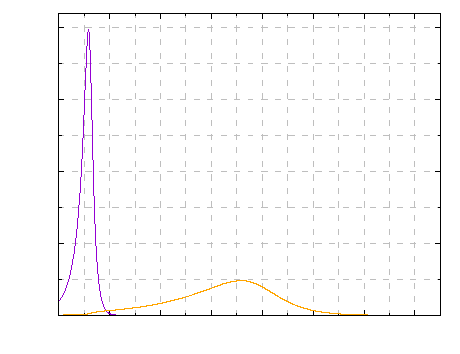
\includegraphics{2-potencies}}%
    \gplfronttext
  \end{picture}%
\endgroup
